% =============================================================================
% Projeto : AuditAI Senado: Transparência e Análise Parlamentar com IA
% Arquivo : artigo/latex/artigo_parcial.tex
% Síntese : Artigo parcial (N1) no template SBC - proposta, dataset, análise
%           exploratória, preparação dos dados e resultados parciais.
% Integrantes: Andrey Bezerra Virgínio dos Santos (10420696), Igor Silva
%   Araujo (10428505), Julia Vitória Bomfim do Nascimento (10425604),
%   William Saran dos Santos Junior (10420128)
% Histórico de alterações (data - autor - descrição):
%   - 26/09/2026 - Igor Silva Araujo - Versão do artigo parcial (N1).
% =============================================================================
\documentclass[12pt]{article}

\usepackage{sbc-template}
\usepackage[T1]{fontenc}
\usepackage[utf8]{inputenc}
\usepackage[brazil]{babel}
\usepackage{graphicx,url}
\usepackage{booktabs}
\usepackage{tabularx}
\usepackage{array}
\usepackage{tikz}
\usetikzlibrary{positioning,arrows.meta,fit,backgrounds}
\urlstyle{same}

% Endereço do repositório público do projeto
\newcommand{\githuburl}{\url{https://github.com/igorsa-hub/auditai-senado}}

\newcolumntype{Y}{>{\raggedright\arraybackslash}X}

\sloppy

\title{AuditAI Senado: Transparência e Análise\\ Parlamentar com IA}

\author{Andrey Bezerra Virgínio dos Santos\inst{1}, Igor Silva Araujo\inst{1},\\
  Julia Vitória Bomfim do Nascimento\inst{1}, William Saran dos Santos Junior\inst{1}}

\address{Faculdade de Computação e Informática -- Universidade Presbiteriana Mackenzie\\
  São Paulo -- SP -- Brasil
  \email{\{10420696, 10428505, 10425604, 10420128\}@mackenzista.com.br}
  \\[4pt]{\footnotesize (e-mails na ordem dos autores; o prefixo de cada e-mail é o RA do integrante)}
}

\begin{document}

\maketitle

\begin{abstract}
  The Brazilian Federal Senate publishes tens of thousands of floor speeches, but their volume
  makes it hard to find which senators address a given issue and where the evidence is. This
  partial paper presents AuditAI Senado, an intelligent agent based on Natural Language
  Processing, semantic search and retrieval-augmented generation (RAG) that will answer
  natural-language questions by grouping speeches per senator and citing excerpts as evidence.
  At this stage, a public dataset with 100,667 speech records (1994--2024) was characterized,
  revealing quality and authorship-attribution issues, and a base of 558,569 excerpts was built.
  A lexical probe showed that literal search misses more than half of the speeches on an example
  topic and suffers from vocabulary drift.
\end{abstract}

\begin{resumo}
  O Senado Federal publica dezenas de milhares de pronunciamentos, mas o volume dificulta
  identificar quais parlamentares abordam um tema e onde estão as evidências. Este artigo parcial
  apresenta o AuditAI Senado, um agente inteligente baseado em Processamento de Linguagem
  Natural, busca semântica e geração aumentada por recuperação (RAG) que responderá a perguntas
  em linguagem natural agrupando discursos por parlamentar e citando trechos como evidência.
  Nesta etapa, caracterizou-se um \textit{dataset} público com 100.667 registros (1994--2024),
  revelando problemas de qualidade e de atribuição de autoria, e construiu-se uma base de 558.569
  trechos. Uma sondagem léxica mostrou que a busca literal perde mais da metade dos discursos de
  um tema-exemplo e sofre com a deriva de vocabulário.
\end{resumo}

% -----------------------------------------------------------------------------
\section{Introdução}

\subsection{Contextualização}

A Lei de Acesso à Informação \cite{brasil2011} consolidou no Brasil o princípio de que a
informação produzida pelo Estado deve ser pública. No Poder Legislativo, isso se traduz na
publicação, em portais oficiais, dos pronunciamentos feitos pelos parlamentares. O Senado Federal
disponibiliza em seu portal o texto de dezenas de milhares desses discursos, cobrindo três
décadas de atividade legislativa. Contudo, \emph{acesso} não é o mesmo que \emph{compreensão}: o
conjunto de dados utilizado neste projeto reúne mais de cem mil registros e cerca de 107 milhões
de palavras atribuídas aos autores dos discursos --- volume impossível de ser lido por um
cidadão, jornalista ou pesquisador interessado em saber, por exemplo, quais senadores mais se
dedicaram a debater violência contra a mulher, meio ambiente ou inteligência artificial, e o que
efetivamente disseram.

As ferramentas usuais de consulta dependem da ocorrência literal de palavras. Porém, um mesmo
assunto pode ser expresso de muitas formas (``violência doméstica'', ``feminicídio'', ``Lei Maria
da Penha'') e o vocabulário muda ao longo do tempo. O problema tratado neste trabalho é, portanto,
o de \textbf{recuperar e organizar automaticamente, por significado, os discursos parlamentares
relacionados a um tema, atribuindo-os corretamente aos seus autores e apresentando as evidências
textuais}. O projeto insere-se no Objetivo de Desenvolvimento Sustentável 16 --- Paz, Justiça e
Instituições Eficazes \cite{onu2015} ---, em particular nas metas de instituições transparentes
(16.6) e de acesso público à informação (16.10).

\subsection{Justificativa}

Como os dados são textos em linguagem natural, o problema pertence ao campo do Processamento de
Linguagem Natural (PLN). Métodos léxicos, como o BM25 \cite{robertson2009}, são eficientes, mas
só encontram documentos que compartilham termos com a consulta. Representações vetoriais densas
(\textit{embeddings}) produzidas por modelos baseados em \textit{Transformers}
\cite{vaswani2017,reimers2019,wang2024e5} aproximam textos pelo significado e permitem a
\textbf{busca semântica}. Para produzir respostas legíveis, um modelo de linguagem de grande
escala (LLM) pode redigir a resposta; porém, LLMs podem gerar afirmações sem respaldo
(``alucinações'') \cite{ji2023}. A arquitetura de geração aumentada por recuperação (RAG)
\cite{lewis2020} mitiga esse risco ao condicionar a resposta aos trechos recuperados, que são
exibidos como fonte. Por fim, perguntas como ``quais parlamentares mais abordaram X entre 2015 e
2020?'' exigem uma sequência de operações (interpretar a intenção, buscar, filtrar, agrupar por
parlamentar, selecionar evidências), o que justifica organizar a solução como um \textbf{agente
inteligente} \cite{russell2022} capaz de escolher e encadear ferramentas \cite{yao2023}.
A solução também distinguirá explicitamente \emph{mencionar} um tema de \emph{assumir uma posição}
sobre ele, pois a ocorrência de um assunto num discurso não revela, por si só, o posicionamento
político do parlamentar.

\subsection{Motivação}

Do ponto de vista social, a ferramenta reduz o custo de acompanhar a atuação discursiva dos
representantes eleitos, apoiando o controle social, o jornalismo de dados e a pesquisa em ciência
política --- área em que o uso de textos como dados já é consolidado, mas exige validação
cuidadosa dos métodos automáticos \cite{grimmer2013}. Do ponto de vista acadêmico, o projeto
permite aplicar, em um corpus real e extenso em português, conceitos centrais da disciplina: PLN,
recuperação de informação, modelos de linguagem, RAG e agentes. Do ponto de vista prático, o
problema é bem delimitado, os dados são públicos e o resultado --- um protótipo que responde com
evidências verificáveis --- é demonstrável e avaliável.

\subsection{Objetivo}

O objetivo geral é \textbf{desenvolver um agente inteligente capaz de responder a perguntas em
linguagem natural sobre os temas abordados nos discursos do Senado Federal, identificando os
discursos semanticamente relacionados à consulta, agrupando os resultados por parlamentar e
apresentando trechos que fundamentem a resposta, com ligação para a fonte oficial}. Os objetivos
específicos são:
(i) caracterizar e preparar a base textual de discursos (1º bimestre);
(ii) implementar e comparar estratégias de recuperação léxica (BM25), densa (\textit{embeddings})
e híbrida;
(iii) integrar a recuperação a um agente com LLM em arquitetura RAG, que agrupe resultados por
parlamentar e cite evidências;
(iv) avaliar a qualidade da recuperação e a fidelidade das respostas; e
(v) disponibilizar uma interface web para consulta (itens ii a v no 2º bimestre).

\subsection{Contribuições esperadas}

Seguindo as dimensões de contribuição definidas na proposta, espera-se:
(a) \emph{compreensão do problema} --- formalizar ``quem fala sobre o quê'' como uma tarefa de
recuperação de trechos seguida de agregação por autor;
(b) \emph{dados} --- uma base de discursos caracterizada, limpa e segmentada, com os problemas de
qualidade documentados (entregue nesta etapa);
(c) \emph{modelagem, experimentação e avaliação} --- comparação quantitativa entre recuperação
léxica, densa e híbrida sobre um conjunto de perguntas com julgamentos de relevância;
(d) \emph{aplicação} --- um protótipo funcional do agente com interface web;
(e) \emph{explicabilidade} --- respostas sempre acompanhadas das evidências que as sustentam;
(f) \emph{reprodutibilidade} --- código, notebooks e documentação em repositório público; e
(g) \emph{análise crítica} --- discussão de vieses, limitações e riscos do uso de IA na análise de
conteúdo político.

% -----------------------------------------------------------------------------
\section{Fundamentação Teórica}

\subsection{Processamento de Linguagem Natural e recuperação de informação}

O PLN estuda métodos computacionais para analisar e gerar linguagem humana
\cite{jurafsky2025}. Em recuperação de informação, o modelo clássico representa documentos como
``sacos de palavras'' ponderados, por exemplo pelo TF-IDF, que valoriza termos frequentes no
documento e raros na coleção \cite{manning2008}. O BM25 refina essa ideia com saturação da
frequência do termo e normalização pelo tamanho do documento, sendo até hoje uma linha de base
forte \cite{robertson2009}. A principal limitação desses métodos é o \emph{descasamento de
vocabulário}: documentos relevantes que não usam as palavras da consulta não são encontrados. A
avaliação costuma usar métricas de ranqueamento como Recall@$k$, MRR (\textit{Mean Reciprocal
Rank}) e nDCG (\textit{normalized Discounted Cumulative Gain}) \cite{manning2008}.

\subsection{\textit{Embeddings} e busca semântica}

A arquitetura \textit{Transformer}, baseada em mecanismos de atenção \cite{vaswani2017}, deu
origem a modelos de linguagem pré-treinados que produzem representações contextuais do texto,
inclusive para o português, como o BERTimbau \cite{souza2020}. Para comparar sentenças e
parágrafos de forma eficiente, o Sentence-BERT \cite{reimers2019} treina redes siamesas que
mapeiam cada texto para um vetor de dimensão fixa, de modo que textos com significado próximo
fiquem próximos no espaço vetorial (medido, por exemplo, pela similaridade do cosseno). Modelos
multilíngues treinados por aprendizado contrastivo, como a família multilingual-E5
\cite{wang2024e5}, estendem essa capacidade a dezenas de idiomas. Na \emph{recuperação densa}
\cite{karpukhin2020}, consulta e documentos são codificados como vetores e a busca retorna os
vizinhos mais próximos da consulta em um índice vetorial. Como esses modelos têm limite de
entrada (tipicamente 512 \textit{tokens}), documentos longos são divididos em trechos
(\textit{chunks}).

\subsection{Modelos de linguagem e geração aumentada por recuperação}

LLMs geram texto fluente, mas seu conhecimento é limitado aos dados de treinamento e podem
produzir conteúdo não fundamentado \cite{ji2023}. A abordagem RAG \cite{lewis2020} combina um
\emph{recuperador}, que seleciona trechos relevantes de uma base externa, e um \emph{gerador}, que
redige a resposta condicionada a esses trechos. Além de reduzir alucinações, a RAG torna a
resposta auditável, pois as fontes utilizadas podem ser exibidas ao usuário --- requisito central
em um sistema de transparência.

\subsection{Agentes inteligentes}

Um agente é uma entidade que percebe seu ambiente e age sobre ele para atingir objetivos
\cite{russell2022}. Agentes baseados em LLM usam o modelo para decidir quais ações (ferramentas)
executar; o padrão ReAct \cite{yao2023} intercala passos de raciocínio e de ação, observando o
resultado de cada ação antes de decidir a próxima. No AuditAI Senado, o ambiente é a base de
discursos, as percepções são a pergunta do usuário e os resultados das ferramentas, e as ações
são operações como busca temática, aplicação de filtros (período, partido), agrupamento por
parlamentar e recuperação de evidências.

\subsection{Trabalhos relacionados}

\cite{moreira2020} analisou mais de
127 mil pronunciamentos da Câmara dos Deputados (1999--2014) com um modelo de agenda expressa (um
modelo de tópicos) e mostrou que a ênfase temática dos deputados não é explicada principalmente
pela dinâmica governo--oposição, mas por fatores como ideologia, gênero e popularidade. O
trabalho evidencia o valor dos discursos como dado sobre a agenda parlamentar, mas produz
análises agregadas, não respostas a perguntas com evidências.

\cite{soriano2026} mapearam 453.280 discursos da Câmara (2003--2025) combinando estilometria,
modelagem de tópicos com BERTopic sobre \textit{embeddings} multilíngues, agregação temática
assistida por LLM e agrupamento semântico (UMAP e HDBSCAN), identificando 49 agrupamentos
discursivos que atravessam fronteiras partidárias e mostrando a reatividade da agenda a crises. O
estudo confirma que \textit{embeddings} capturam bem temas em discursos políticos em português,
mas tem caráter exploratório e não supervisionado.

\cite{vitorio2022} propuseram o Ulysses-RFSQ, que adiciona ao BM25 um bônus de
\textit{relevance feedback} derivado de consultas semelhantes, em uma base de solicitações
legislativas da Câmara dos Deputados, elevando o Recall@20 do BM25 em quase 3\%. O trabalho mostra
que o BM25 é uma linha de base competitiva em textos legislativos em português.

\cite{sivakumar2026} construíram um sistema RAG de perguntas e respostas sobre 3.500 documentos
do Parlamento indiano (Lok Sabha, 2021--2024), com o modelo \textit{all-MiniLM-L6-v2}, índice FAISS,
trechos de 256 a 512 \textit{tokens} com 15\% de sobreposição e recuperação dos 3 trechos mais
similares. A acurácia factual subiu de 80\% (gerador sem recuperação) para 94\% com RAG; entre as
principais causas de erro estavam o raciocínio em múltiplas etapas e o contexto recuperado
incompleto --- o que reforça a importância de avaliar a recuperação separadamente.

\cite{cunha2026} avaliaram de ponta a ponta um sistema RAG para documentos hospitalares em
português, com o modelo multilingual-E5-small, trechos de cerca de 100 \textit{tokens}, fusão de
rankings por \textit{Reciprocal Rank Fusion} (RRF) e comparação de geradores. O sistema obteve MRR
de 0,786 e nDCG@10 de 0,816 em 192 pares de pergunta--resposta, com validação por especialistas.

A Tabela~\ref{tab:relacionados} sintetiza os trabalhos e as decisões que eles fundamentam neste
projeto. Nenhum deles trata do Senado Federal com respostas que \emph{agregam resultados por
parlamentar} e apresentam as evidências; os trabalhos sobre discursos são descritivos, e os
sistemas RAG respondem a perguntas factuais pontuais. Além disso, nenhum discute a atribuição de
autoria por papel de fala --- aspecto que, como mostra a Seção~\ref{sec:eda}, afeta cerca de 18\%
das palavras do corpus usado aqui.

\begin{table}[ht]
\centering
\caption{Síntese dos trabalhos relacionados e decisões adotadas no AuditAI Senado.}
\label{tab:relacionados}
\footnotesize
\begin{tabularx}{\textwidth}{@{}>{\raggedright\arraybackslash}p{2.5cm}>{\raggedright\arraybackslash}p{2.6cm}Y Y@{}}
\toprule
\textbf{Trabalho} & \textbf{Dados} & \textbf{Técnica e resultado} & \textbf{Decisão adotada} \\
\midrule
Moreira (2020) & 127 mil discursos, Câmara, 1999--2014 & Modelo de tópicos; ênfase temática ligada a ideologia, gênero, popularidade & Discursos como evidência da agenda; análise por parlamentar \\
Soriano et al. (2026) & 453 mil discursos, Câmara, 2003--2025 & BERTopic, \textit{embeddings}, HDBSCAN; 49 agrupamentos & Uso de \textit{embeddings} multilíngues para temas em português \\
Vitório et al. (2022) & Solicitações legislativas, Câmara & BM25 + \textit{relevance feedback}; +3\% Recall@20 & BM25 como linha de base léxica \\
Sivakumar e Meenakshi (2026) & 3.500 docs., Lok Sabha & RAG (MiniLM + FAISS); acurácia 80\%$\rightarrow$94\% & Trechos com sobreposição; avaliar a recuperação \\
da Cunha et al. (2026) & Docs. hospitalares em português & RAG (E5 + RRF); MRR 0,786, nDCG@10 0,816 & E5 multilíngue, fusão híbrida (RRF), MRR/nDCG \\
\bottomrule
\end{tabularx}
\end{table}

% -----------------------------------------------------------------------------
\section{Metodologia e Resultados Esperados}

\subsection{Abordagem, etapas e resultados esperados}

A solução segue o \textit{pipeline} da Figura~\ref{fig:pipeline}, organizado em sete etapas. As
etapas E1 a E3 correspondem ao 1º bimestre e foram concluídas (Seções~\ref{sec:dataset} a
\ref{sec:parciais}); as etapas E4 a E7 serão desenvolvidas no 2º bimestre.

\begin{itemize}
  \item \textbf{E1 -- Aquisição e caracterização}: obtenção do \textit{dataset} e documentação de
  sua origem, estrutura e licença.
  \item \textbf{E2 -- Análise exploratória}: cobertura temporal, qualidade, distribuições e
  sondagem léxica dos temas-exemplo.
  \item \textbf{E3 -- Preparação}: limpeza, filtros de qualidade e segmentação do texto autoral em
  trechos com metadados.
  \item \textbf{E4 -- Indexação}: índice léxico BM25 e índice vetorial com \textit{embeddings} de
  um modelo multilíngue (candidato principal: multilingual-E5 \cite{wang2024e5}).
  \item \textbf{E5 -- Agente}: um LLM interpreta a pergunta (tema, período, partido, tipo de
  pergunta) e aciona as ferramentas \emph{buscar\_trechos}, \emph{filtrar},
  \emph{agrupar\_por\_parlamentar} e \emph{obter\_evidências}; a resposta final é gerada em
  arquitetura RAG, usando apenas os trechos recuperados e citando-os.
  \item \textbf{E6 -- Interface}: aplicação web que exibe a resposta, o ranking de parlamentares
  (contagem e proporção de discursos) e os trechos com ligação para a página oficial.
  \item \textbf{E7 -- Avaliação}: protocolo descrito a seguir.
\end{itemize}

\begin{figure}[ht]
\centering
\begin{tikzpicture}[
  node distance=4mm and 5mm,
  box/.style={draw, rounded corners=2pt, align=center, font=\sffamily\scriptsize,
              minimum height=9mm, text width=2.15cm, fill=white},
  n1/.style={box, fill=gray!12},
  arr/.style={-{Stealth[length=2mm]}, thick}]
  \node[n1] (d) {E1 \textit{Dataset}\\Kaggle (JSON)};
  \node[n1, right=of d] (e) {E2 Análise\\exploratória};
  \node[n1, right=of e] (p) {E3 Limpeza, filtros\\e trechos};
  \node[box, right=of p] (i) {E4 Índices BM25\\+ vetorial};
  \node[box, below=9mm of i] (a) {E5 Agente\\(LLM + ferramentas)};
  \node[box, left=of a] (g) {Geração RAG\\com citações};
  \node[box, left=of g] (u) {E6 Interface\\web};
  \node[box, left=of u] (v) {E7 Avaliação\\(métricas)};
  \node[box, above=5mm of i, text width=2.4cm, fill=white, draw=gray] (q) {Pergunta do usuário};
  \draw[arr] (d) -- (e); \draw[arr] (e) -- (p); \draw[arr] (p) -- (i);
  \draw[arr] (q) -- (i);
  \draw[arr] (i) -- node[right, font=\sffamily\tiny, align=left]{trechos +\\metadados} (a);
  \draw[arr] (a) -- (g); \draw[arr] (g) -- (u); \draw[arr] (u) -- (v);
\end{tikzpicture}
\caption{Pipeline do AuditAI Senado. Etapas em cinza: concluídas no 1º bimestre.}
\label{fig:pipeline}
\end{figure}

\textbf{Protocolo de avaliação (E7).} Será montado um conjunto de 20 a 30 perguntas temáticas
(incluindo os temas da Tabela~\ref{tab:temas}). Para cada pergunta, os trechos mais bem
ranqueados por BM25, busca densa e busca híbrida (RRF) serão reunidos e julgados como relevantes
ou não por pelo menos dois integrantes, com discussão dos casos de discordância. A recuperação
será comparada por Recall@$k$, MRR e nDCG@10, seguindo \cite{cunha2026} e \cite{vitorio2022}; as
respostas geradas serão verificadas quanto à \emph{fidelidade} (toda afirmação deve estar
sustentada por um trecho citado) e à correção das citações. A tabela de contagens léxicas obtida
nesta etapa (Tabela~\ref{tab:baseline}) servirá como linha de base.

\textbf{Resultados esperados.} Espera-se que a busca semântica ou híbrida supere a léxica em
revocação para temas com vocabulário variado, que as respostas do agente apresentem apenas
afirmações sustentadas por evidências e que o protótipo permita, em poucos segundos, obter a lista
de parlamentares que mais abordaram um tema, com contagem, proporção e trechos verificáveis.

\subsection{\textit{Dataset}: origem, conteúdo e licença}\label{sec:dataset}

Utiliza-se o conjunto público \textit{Brazilian Senate Speeches} \cite{licolabres2024},
disponível no Kaggle sob licença CC BY-NC-SA 4.0 (uso não comercial, com atribuição). Segundo o
autor, os textos foram coletados do portal do Senado a partir das URLs fornecidas pela API de
dados abertos, com raspagem de mais de 100 mil páginas. Foi usada a versão LITE
(\texttt{fsdb\_lite.json}, 934,9~MB), além de dois arquivos auxiliares:
\texttt{partidos.json} (656 senadores e respectivo partido) e \texttt{externos.json} (1.292
nomes de oradores que não seriam senadores). A estrutura de cada registro é apresentada na
Tabela~\ref{tab:estrutura}. Um aspecto decisivo é que o texto é separado por \emph{papel de
fala}: somente o texto \textbf{Autoral} pertence ao autor do pronunciamento.

\begin{table}[ht]
\centering
\caption{Estrutura de um registro do arquivo \texttt{fsdb\_lite.json}.}
\label{tab:estrutura}
\footnotesize
\begin{tabularx}{\textwidth}{@{}p{4.0cm}Y@{}}
\toprule
\textbf{Campo} & \textbf{Conteúdo} \\
\midrule
chave do registro & código do pronunciamento no portal do Senado \\
\texttt{URL}, \texttt{Data} & endereço da página oficial e data do discurso \\
\texttt{Autor} & código, nome simplificado (minúsculas, sem acentos) e partido na data \\
\texttt{Texto.Autoral} & parágrafos falados pelo autor do pronunciamento \\
\texttt{Texto.Apartes} & intervenções de outros senadores durante o discurso \\
\texttt{Texto.Presidencial} & falas de quem preside a sessão \\
\texttt{Texto.Externos} & falas de não-senadores (ministros, convidados) \\
\bottomrule
\end{tabularx}
\end{table}

Os dados foram lidos em \textit{streaming} (biblioteca \texttt{ijson}), em lotes, para evitar
carregar o JSON inteiro em memória. Não foi aplicada anonimização: os registros são atos públicos
de agentes públicos no exercício do mandato, divulgados oficialmente em cumprimento à LAI
\cite{brasil2011}. Ainda assim, adotou-se a minimização de dados: as falas de terceiros
(\textit{Externos}) não são indexadas (ver Seção~\ref{sec:etica}).

\subsection{Análise exploratória}\label{sec:eda}

A análise, reproduzível no notebook do repositório, produziu os seguintes achados.

\textbf{Cobertura temporal.} O \textit{dataset} contém 100.667 registros de 486 parlamentares.
Embora a descrição mencione o período 1988--2024, a cobertura efetiva vai de 1994 a 7 de março
de 2024 (Figura~\ref{fig:ano}): há apenas um registro de 1980 e um de 1988 (datas atípicas), e
1994 (414 registros) e 2024 (258) são anos parciais. Nos anos completos, a média é de 3.448
discursos por ano, com máximo em 2005 (5.375) e mínimo em 2020 (849), ano das sessões remotas da
pandemia. Vários anos de eleições gerais (1998, 2002, 2010, 2014, 2018) estão entre os de menor
produção. Assim, contagens temporais de menções precisarão ser normalizadas pelo volume anual.

\begin{figure}[ht]
\centering
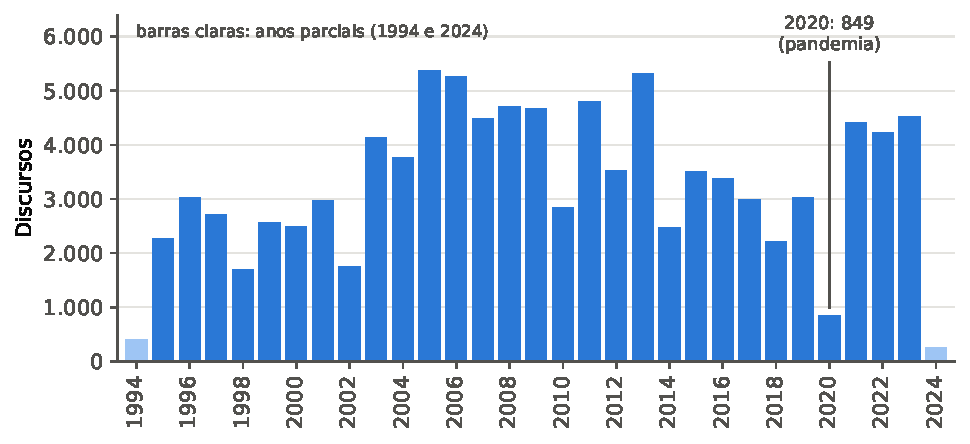
\includegraphics[width=.92\textwidth]{figuras/fig1_discursos_por_ano.pdf}
\caption{Número de discursos por ano no \textit{dataset}.}
\label{fig:ano}
\end{figure}

\textbf{Registros sem texto autoral.} 9.979 registros (9,9\%) não possuem texto autoral; em
67,5\% deles há falas classificadas como \textit{Presidencial}, ou seja, o parlamentar presidia a
sessão. Esses registros não podem ser atribuídos como discurso do parlamentar e foram excluídos
da base de busca.

\textbf{Composição por papel de fala.} Do total de palavras, 81,9\% são autorais, 14,2\% são
apartes, 3,1\% são falas da Presidência e 0,8\% de oradores externos; 25,9\% dos registros contêm
apartes. Indexar o texto completo atribuiria ao autor cerca de 18\% de palavras ditas por outras
pessoas --- um erro de atribuição inaceitável num sistema de transparência. Por isso apenas o
texto autoral é utilizado.

\textbf{Autores e a lista de externos.} Ao testar o filtro sugerido pelo autor do
\textit{dataset}, verificou-se que 629 registros, de 35 autores, seriam removidos por constarem
em \texttt{externos.json}; a inspeção mostrou tratar-se de parlamentares que exerceram mandato no
Senado (vários suplentes). Como o campo \texttt{Autor} vem do registro oficial, a lista
\emph{não} foi usada como filtro. Também foram encontrados 380 textos autorais idênticos sob
códigos distintos. Os identificadores são consistentes: cada código de autor corresponde a um
único nome.

\textbf{Concentração.} Entre os 481 autores com texto autoral, a mediana é de 81 discursos por
autor, mas os 10\% mais ativos (49 senadores) respondem por 47,3\% dos discursos. Um ranking por
contagem absoluta tenderia, portanto, a favorecer quem mais discursa em geral.

\textbf{Partidos.} Há 61 rótulos de partido, reduzidos a 42 após corrigir apenas variações de
grafia (espaços, ``PC DO B''/``PCdoB'', ``PODE''/``PODEMOS''). Renomeações históricas (PMDB$\rightarrow$MDB,
PFL$\rightarrow$DEM$\rightarrow$UNIÃO etc.) foram mantidas, pois o campo registra o partido na data do discurso.

\textbf{Tamanho dos discursos.} A distribuição do número de palavras autorais é assimétrica
(Figura~\ref{fig:tamanho}): mediana de 978, quartis de 442 e 1.649 e máximo de 29.586 palavras. A
cauda curta é dominada por manifestações procedimentais (``o partido orienta o voto sim''),
enquanto discursos longos excedem o limite de entrada dos modelos de \textit{embeddings} --- o que
motiva a segmentação em trechos. Os termos mais frequentes, mesmo após remover
\textit{stopwords}, são de tratamento e procedimento (\textit{presidente}, \textit{senador},
\textit{governo}), indicando que representações por frequência de palavras tendem a capturar o
``ritual'' parlamentar e não o tema.

\begin{figure}[ht]
\centering
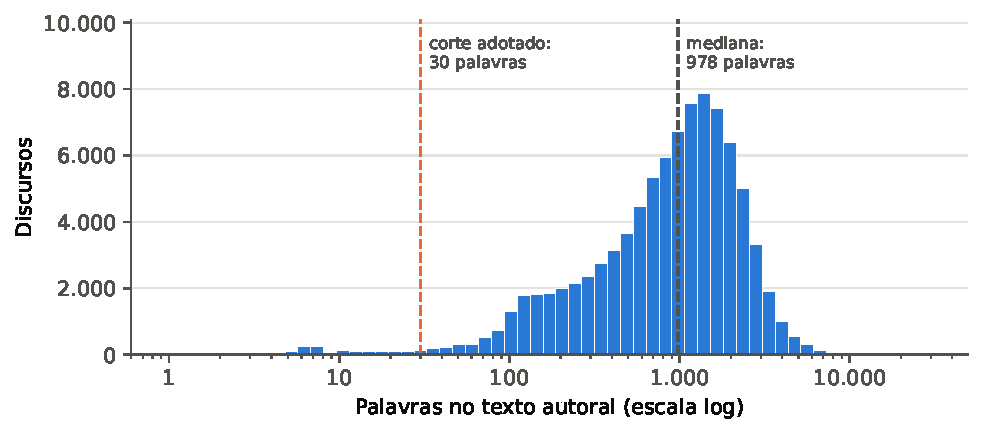
\includegraphics[width=.92\textwidth]{figuras/fig3_tamanho_discursos.pdf}
\caption{Distribuição do número de palavras do texto autoral (escala logarítmica).}
\label{fig:tamanho}
\end{figure}

\textbf{Sondagem temática léxica.} Para os temas citados na proposta, comparou-se a busca pela
expressão exata com a busca por um conjunto de termos relacionados definido pelo grupo, em texto
minúsculo e sem acentos (Tabela~\ref{tab:temas}). Para violência contra a mulher, a expressão
exata encontra 815 discursos, contra 1.708 com os termos relacionados (+109,6\%): a busca literal
perde mais da metade dos discursos. Em temas amplos, como educação e saúde, os termos aparecem em
cerca de 30\% a 35\% de todo o corpus, muitas vezes de passagem, de modo que a simples ocorrência
não indica que o discurso trate do tema. ``Inteligência artificial'' é raro (75 discursos).

\begin{table}[ht]
\centering
\caption{Discursos encontrados por busca léxica, por tema (base de 90.688 discursos com texto autoral).}
\label{tab:temas}
\footnotesize
\begin{tabular}{@{}lrrrr@{}}
\toprule
\textbf{Tema} & \textbf{Expressão exata} & \textbf{Termos relacionados} & \textbf{Acréscimo} & \textbf{\% do corpus} \\
\midrule
Violência contra a mulher & 815    & 1.708  & +109,6\% & 1,9\% \\
Meio ambiente             & 7.221  & 9.379  & +29,9\%  & 10,3\% \\
Inteligência artificial   & 75     & 75     & 0,0\%    & 0,1\% \\
Educação                  & 21.240 & 31.626 & +48,9\%  & 34,9\% \\
Saúde                     & 23.451 & 26.729 & +14,0\%  & 29,5\% \\
\bottomrule
\end{tabular}
\end{table}

A Figura~\ref{fig:termos} mostra a \emph{deriva de vocabulário}: ``feminicídio'' é praticamente
ausente até 2012, cresce a partir de 2013 --- período de tramitação do projeto que resultou na Lei
13.104/2015 --- e supera a expressão genérica em 2020 e 2023; ``inteligência artificial'' passa de
0,20\% dos discursos em 2018 para 0,76\% em 2023 (o pico de 2020 decorre, em parte, do pequeno
número de discursos naquele ano). Uma busca com vocabulário fixo fica, portanto, defasada ao longo
de três décadas, o que reforça a necessidade de recuperação por significado.

\begin{figure}[ht]
\centering
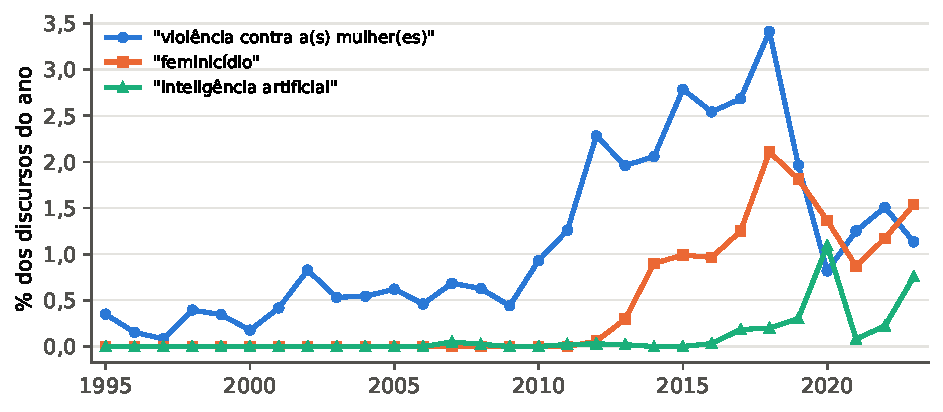
\includegraphics[width=.92\textwidth]{figuras/fig4_evolucao_termos.pdf}
\caption{Percentual anual de discursos que mencionam cada expressão (1995--2023).}
\label{fig:termos}
\end{figure}

\subsection{Preparação dos dados}\label{sec:preparacao}

A preparação, implementada nos módulos \texttt{carregamento.py} e \texttt{preparacao.py}, teve
quatro passos.
(1) \emph{Limpeza}: normalização Unicode (NFC), remoção de rótulos de orador e de cabeçalhos que
sobraram da página (``O SR. FULANO (PARTIDO -- UF) --'', ``Sem revisão do orador'') e de
anotações taquigráficas, e normalização de espaços; 1.242 textos foram alterados. Acentos e
\textit{stopwords} foram preservados no texto destinado aos \textit{embeddings}, pois os modelos
de linguagem utilizam essa informação; a versão minúscula e sem acentos é usada apenas na busca
léxica.
(2) \emph{Normalização de siglas partidárias}, conforme descrito na Seção~\ref{sec:eda}.
(3) \emph{Filtros de qualidade} (Tabela~\ref{tab:filtros}): remoção de registros sem texto
autoral, de textos duplicados (por \textit{hash} MD5) e de discursos com menos de 30 palavras,
limiar definido por inspeção manual da cauda curta. Os dois registros com datas atípicas não
tinham texto autoral e foram eliminados no primeiro filtro.
(4) \emph{Segmentação}: cada texto autoral foi dividido em trechos de até 250 palavras formados
por sentenças inteiras, com sobreposição de até 50 palavras entre trechos vizinhos. A faixa é
compatível com os trabalhos relacionados (100 a 512 \textit{tokens}, 15\% a 20\% de sobreposição)
e tende a respeitar o limite de 512 \textit{tokens} de modelos como o multilingual-E5; a contagem
exata em \textit{tokens} será verificada na E4 com o \textit{tokenizer} do modelo escolhido. Cada
trecho herda código, data, autor, partido e URL do discurso, o que permite agrupar resultados por
parlamentar e citar a fonte.

\begin{table}[ht]
\centering
\caption{Efeito dos filtros de qualidade sobre a base.}
\label{tab:filtros}
\footnotesize
\begin{tabular}{@{}lrr@{}}
\toprule
\textbf{Etapa} & \textbf{Removidos} & \textbf{Restantes} \\
\midrule
Registros originais                        & --    & 100.667 \\
Sem texto autoral                          & 9.979 & 90.688 \\
Texto autoral duplicado                    & 385   & 90.303 \\
Menos de 30 palavras (procedimentais)      & 1.286 & 89.017 \\
\bottomrule
\end{tabular}
\end{table}

A base final contém \textbf{89.017 discursos} de 481 parlamentares (03/01/1994 a 07/03/2024),
segmentados em \textbf{558.569 trechos}, com mediana de 5 trechos por discurso e de 235 palavras
por trecho; 14,1\% dos discursos cabem em um único trecho.

% -----------------------------------------------------------------------------
\section{Resultados Parciais}\label{sec:parciais}

\subsection{Aspectos éticos e responsabilidade no uso da IA}\label{sec:etica}

Uma ferramenta que associa parlamentares a temas tem impacto potencial sobre a reputação de
pessoas públicas e sobre o debate político. Os riscos identificados a partir dos dados e das
técnicas escolhidas, bem como as medidas adotadas ou planejadas, estão na
Tabela~\ref{tab:etica}, alinhadas aos princípios de transparência, responsabilização e
supervisão humana da recomendação da UNESCO sobre ética da IA \cite{unesco2021}.

\begin{table}[ht]
\centering
\caption{Riscos éticos do AuditAI Senado e medidas de mitigação.}
\label{tab:etica}
\footnotesize
\begin{tabularx}{\textwidth}{@{}p{3.1cm}YY@{}}
\toprule
\textbf{Risco} & \textbf{Onde aparece no projeto} & \textbf{Mitigação} \\
\midrule
Atribuição indevida de falas & 18\% das palavras de um registro são de outros oradores & Indexar só o texto autoral (adotado) \\
Confundir menção com posição & Um discurso pode citar um tema para defendê-lo ou criticá-lo & Não inferir posicionamento; exibir o trecho e aviso explícito na interface \\
Viés de volume e de cobertura & 10\% mais ativos concentram 47,3\% dos discursos; 9,9\% dos registros sem texto; 2020 atípico & Mostrar contagem \emph{e} proporção; declarar lacunas e período coberto \\
Alucinação do LLM & Geração de respostas na etapa RAG & Responder só com trechos recuperados, citar a fonte, responder ``não encontrado'' quando não houver evidência \\
Viés dos modelos e do texto & Transcrições antigas com erros de grafia; vieses de \textit{embeddings} e LLMs & Avaliação por tema e período; análise de erros na N2 \\
Uso político seletivo & Recortes podem ser usados fora de contexto & Ligação para o discurso completo; sem notas ou ``pontuações'' de parlamentares \\
Privacidade & Falas de cidadãos convidados (\textit{Externos}) & Minimização: falas de terceiros não indexadas; licença não comercial respeitada \\
\bottomrule
\end{tabularx}
\end{table}

Quanto à privacidade, os dados são públicos e referem-se a atos oficiais; a LGPD admite o
tratamento de dados de acesso público desde que respeitados a finalidade, a boa-fé e o interesse
público que justificaram sua disponibilização \cite{brasil2018}. O propósito do projeto ---
facilitar o controle social --- é coerente com essa finalidade. A responsabilidade pelas decisões
de projeto é do grupo: código, dados derivados, parâmetros e limitações ficam documentados no
repositório, e o sistema será apresentado como ferramenta de apoio à consulta, sempre sujeita à
verificação humana das fontes.

\subsection{Resultados parciais obtidos}

As etapas previstas para o 1º bimestre (E1 a E3) foram concluídas e produziram:
(i) a caracterização do \textit{dataset}, que corrigiu o período declarado na proposta
(1994--2024) e revelou problemas de qualidade não documentados pelo autor dos dados --- registros
sem texto autoral, falas de terceiros misturadas aos registros, duplicatas, datas atípicas,
variações de grafia de partidos e a inadequação da lista de externos como filtro;
(ii) evidências quantitativas de que a busca literal é insuficiente (perda de mais da metade dos
discursos do tema-exemplo e deriva de vocabulário ao longo do tempo), que sustentam a escolha da
busca semântica;
(iii) uma base de 558.569 trechos com metadados, pronta para a indexação da etapa E4; e
(iv) uma linha de base léxica para a pergunta-exemplo da proposta.

A Tabela~\ref{tab:baseline} mostra essa linha de base: os parlamentares com mais discursos que
contêm termos relacionados a violência contra a mulher (1.708 discursos de 211 autores). A coluna de
proporção altera a leitura: parlamentares com menos discursos no total dedicaram ao tema uma
fração muito maior de sua atuação. Esse é o tipo de resposta que o agente deverá fornecer ---
agora com recuperação semântica, descarte de menções de passagem e exibição dos trechos. Os
resultados são contagens de menções e \emph{não} indicam posicionamento.

\begin{table}[ht]
\centering
\caption{Linha de base léxica: parlamentares com mais discursos que mencionam termos de violência contra a mulher (nomes conforme o campo \texttt{NomeSimples}, sem acentos).}
\label{tab:baseline}
\footnotesize
\begin{tabular}{@{}lrrr@{}}
\toprule
\textbf{Parlamentar} & \textbf{Discursos com menção} & \textbf{Total de discursos} & \textbf{Proporção} \\
\midrule
Paulo Paim          & 193 & 3.055 & 6,3\% \\
Vanessa Grazziotin  & 96  & 1.068 & 9,0\% \\
Angela Portela      & 83  & 628   & 13,2\% \\
Serys Slhessarenko  & 64  & 476   & 13,4\% \\
Ana Rita            & 56  & 176   & 31,8\% \\
\bottomrule
\end{tabular}
\end{table}

\textbf{Limitações observadas.} A cobertura depende da raspagem feita pelo autor do
\textit{dataset}; registros de parlamentares presidindo sessões ficam fora da base; transcrições
antigas contêm erros de grafia e trechos sem acentuação, o que pode reduzir a revocação para
períodos mais antigos; e a lista de termos relacionados da sondagem léxica reflete escolhas do
grupo, servindo como indício, não como verdade de referência.

\subsection{Repositório GitHub}

Todo o material está disponível publicamente em \githuburl: o artigo (PDF e fonte
\LaTeX), a descrição do \textit{dataset} com instruções de obtenção e amostras dos dados
preparados, o notebook executado da análise exploratória e da preparação, os módulos Python
(\texttt{src/}) com cabeçalho de identificação e histórico de alterações, as figuras, as tabelas e
as métricas geradas.

\bibliographystyle{sbc}
\bibliography{referencias}

\end{document}
